%Developed by Konstantinos Xouveroudis - 2020
%Please use XeLaTeX




%Δομή του έγγραφου και μέγευος γραμματοσειράς (10pt, 11pt, ή 12pt).
\documentclass[twoside, a4paper, 11pt]{article}

%Περιθώρια σελίδας και ύψος για το header και footer.
\usepackage[top=2.5cm, left=2.5cm, right=2.5cm, bottom=2.5cm, headheight=1.25cm, footskip=1.25cm]{geometry}

\usepackage[utf8]{inputenc}
\usepackage[T1]{fontenc}
\usepackage[greek,english]{babel}

\usepackage{fontspec}
 
\setmainfont{Times New Roman}


%Μας επιτρέπει να αλλάζουμε από ελληνικά σε αγγλικά και το αντίθετο.
\usepackage{alphabeta}

\usepackage{graphicx}
\graphicspath{ {./Images/} }
%\usepackage{algorithmic}
%\usepackage{algorithm}
\usepackage{adjustbox}
\usepackage{tabularx}
\usepackage{MnSymbol}
%\usepackage{amsfonts}
\usepackage{appendix}
\usepackage{listings}
\usepackage{color}
\usepackage{changepage}
\usepackage{subfigure}
\usepackage{setspace}
\usepackage{fancyhdr} %Κεφαλίδες και υποσέλιδα
\usepackage{url}
\usepackage{multirow}
%\usepackage{indentfirst}
\usepackage{cite}

\setlength{\parindent}{0em}

\usepackage{caption}
\captionsetup[figure]{name=Σχήμα}
\captionsetup[table]{name=Πίνακας}




%\floatname{algorithm}{Αλγόριθμος}

% (1) Βάζει τα tables/figures να αριθμίζονται σύμφωνα με το κεφάλαιο (section).
\usepackage{chngcntr}
\counterwithin{table}{section}
\counterwithin{figure}{section}

% Διαφορετική γραμματοσειρά για τους τίτλους των sections/subsections/subsubsections. Δεν χρειάζεται, αλλά τα αφήνω σε σχόλια.
%\usepackage{titlesec}
%\titleformat*{\section}{\Large\bfseries\sffamily}
%\titleformat*{\subsection}{\large\bfseries\sffamily}
%\titleformat*{\subsubsection}{\large\bfseries\sffamily}

% (2) Settings για την σελίδα αφιερώσεων
\newenvironment{dedication}
  {\clearpage            % Νέα σελίδα
   \thispagestyle{empty} % Χωρίς header/footer
   \vspace*{\stretch{1}} % Κενό στην αρχή της σελίδας
   \itshape              % Italics
   \raggedleft           % Στοίχηση στα δεξιά
  }
  {\par % Τέλος παραγράφου
   \vspace{\stretch{3}} % Κενό στο τέλος της σελίδας, 3 φορές το μέγεθος αυτού στην αρχή.
   \clearpage           % Τέλος σελίδας
}

% (3) Κάνει τα abstracts να έχουν τον τίτλο τους στα αριστερά.
\renewenvironment{abstract}
{\par\noindent\textbf{\abstractname}\\ [0.4cm] \ignorespaces}

% (4) Αλλάζει την δομή των τίτλων των sections ώστε να λένε π.χ. "Κεφάλαιο 1ο: Εισαγωγή".
\usepackage{titlesec}
\titleformat{\section}
{\normalfont\large\bfseries}{Κεφάλαιο~\thesection ο:}{1em}{}

\begin{document}

% (5) Κάνει τον τίτλο του κεφαλαίου να εμφανίζεται στις μονές σελίδες και τον αριθμό 
%\setlength{\headheight}{1.25cm}
\fancypagestyle{custom_page_style}{
  \fancyhf{} % Clear header/footer
  
  \fancyhead[RO]{\nouppercase{\leftmark}} % Τίτλος κεφαλαίου στις μονές σελίδες (γράφει αυτόματα και τον αριθμό)
  \fancyhead[LE]{Κεφάλαιο \thesection} % Αριθμός κεφαλαίου στις ζυγές σελίδες (π.χ. "Κεφάλαιο 1").
  \fancyfoot[C]{\thepage}
  \renewcommand{\headrulewidth}{0pt} % Header rule of .4pt
}

\begin{titlepage}

\newcommand{\HRule}{\rule{\linewidth}{0.6mm}}
\center

\includegraphics[scale=0.6]{Images/ihu-logo-gr.png}\\[1cm]

\textsc{\huge ΣΧΟΛΗ ΜΗΧΑΝΙΚΩΝ}\\

\setstretch{1.5}
\textsc{\huge ΤΜΗΜΑ ΜΗΧΑΝΙΚΩΝ ΠΛΗΡΟΦΟΡΙΚΗΣ \\ ΚΑΙ ΗΛΕΚΤΡΟΝΙΚΩΝ ΣΥΣΤΗΜΑΤΩΝ}\\[1.5cm] % Όνομα της σχολής.

\textsc{\huge ΔΙΠΛΩΜΑΤΙΚΗ ΕΡΓΑΣΙΑ}\\[0.2cm]
{\huge <<ΘΕΜΑ>>}\\[1cm]


\includegraphics[scale=0.8]{Images/Cover-Image-Placeholder.png}\\[1cm]

\setstretch{1}
    \begin{minipage}{0.45\textwidth}
    \begin{flushleft} \large
    \textbf{Τ... φοιτητ.....}
    \\\textbf{........................................} % Όνομα φοιτιτή.
    \\\textbf{Αρ. Μητρώου: ............}
    \end{flushleft}
    \end{minipage}
    ~
    \begin{minipage}{0.45\textwidth}
    \begin{flushright} \large
    \textbf{Επιβλέπων}
    \\\textbf{Ονοματεπώνυμο .......}
    \\\textbf{Βαθμίδα .......}
    \end{flushright}
    \end{minipage}\\[5cm]

{\large \selectlanguage{Greek}\today}\\[2cm]

\end{titlepage}

\clearpage

\pagenumbering{roman} 
\thispagestyle{empty}

\renewcommand{\abstractname}{}
\begin{abstract}
    
\begin{center}
\begin{minipage}{0.9\textwidth}
    \centerline{Τίτλος Δ.Ε. ....}
    \centerline{Κωδικός Δ.Ε. ....}	
    \centerline{Ονοματεπώνυμο φοιτητή/ών ....}
    \centerline{Ονοματεπώνυμο εισηγητή ....}
    \centerline{Ημερομηνία ανάληψης Δ.Ε. ....}
    \centerline{Ημερομηνία περάτωσης Δ.Ε. ....}
\end{minipage}
\end{center}
\selectlanguage{greek}

\setlength{\parskip}{2em}
\emph{Βεβαιώνω ότι είμαι ο συγγραφέας αυτής της εργασίας και ότι κάθε βοήθεια την οποία είχα για την προετοιμασία της είναι πλήρως αναγνωρισμένη και αναφέρεται στην εργασία. Επίσης, έχω καταγράψει τις όποιες πηγές από τις οποίες έκανα χρήση δεδομένων, ιδεών, εικόνων και κειμένου, είτε αυτές αναφέρονται ακριβώς είτε παραφρασμένες. Επιπλέον, βεβαιώνω ότι αυτή η εργασία προετοιμάστηκε από εμένα προσωπικά, ειδικά ως διπλωματική εργασία, στο Τμήμα Μηχανικών Πληροφορικής και Ηλεκτρονικών Συστημάτων του ΔΙ.ΠΑ.Ε.}

\setlength{\parskip}{1em}

\emph{Η παρούσα εργασία αποτελεί πνευματική ιδιοκτησία τ...  φοιτητ... ............................................ που την εκπόνησε/αν. Στο πλαίσιο της πολιτικής ανοικτής πρόσβασης, ο συγγραφέας/δημιουργός εκχωρεί στο Διεθνές Πανεπιστήμιο της Ελλάδος άδεια χρήσης του δικαιώματος αναπαραγωγής, δανεισμού, παρουσίασης στο κοινό και ψηφιακής διάχυσης της εργασίας διεθνώς, σε ηλεκτρονική μορφή και σε οποιοδήποτε μέσο, για διδακτικούς και ερευνητικούς σκοπούς, άνευ ανταλλάγματος. Η ανοικτή πρόσβαση στο πλήρες κείμενο της εργασίας, δεν σημαίνει καθ’ οιονδήποτε τρόπο παραχώρηση δικαιωμάτων διανοητικής ιδιοκτησίας του συγγραφέα/δημιουργού, ούτε επιτρέπει την αναπαραγωγή, αναδημοσίευση, αντιγραφή, πώληση, εμπορική χρήση, διανομή, έκδοση, μεταφόρτωση (downloading), ανάρτηση (uploading), μετάφραση, τροποποίηση με οποιονδήποτε τρόπο, τμηματικά ή περιληπτικά της εργασίας, χωρίς τη ρητή προηγούμενη έγγραφη συναίνεση του συγγραφέα/δημιουργού.}

Η έγκριση της διπλωματικής εργασίας από το Τμήμα Μηχανικών Πληροφορικής και Ηλεκτρονικών Συστημάτων του Διεθνούς Πανεπιστημίου της Ελλάδος, δεν υποδηλώνει απαραιτήτως και αποδοχή των απόψεων του συγγραφέα, εκ μέρους του Τμήματος.

\end{abstract}

\clearpage

\begin{dedication}
<<Αφιέρωση>>
\end{dedication}

% Κενή σελίδα
\newpage
\thispagestyle{empty}
\mbox{}

\clearpage
\large 
\renewcommand{\abstractname}{Πρόλογος}
\begin{abstract}
\addcontentsline{toc}{subsection}{Πρόλογος} %Προσθέτει αυτό το abstract στα περιεχόμενα (table of contents).
\normalsize

Σε αυτήν την ενότητα ο φοιτητής/φοιτήτρια μπορεί να αναφέρει τους λόγους που επέλεξε αυτήν την διπλωματική και το όφελος που είχε. Δεν θα πρέπει να ξεπεράσει τις 200 λέξεις. 

\end{abstract}
\normalsize
\clearpage


\large
\renewcommand{\abstractname}{Περίληψη}
\selectlanguage{greek}
\begin{abstract}
\addcontentsline{toc}{subsection}{Περίληψη} %Πρόσθεση στα περιεχόμενα (table of contents)
\normalsize

Σε αυτήν την ενότητα ο φοιτητής/φοιτήτρια θα πρέπει να περιγράψει συνοπτικά το θέμα και τα αποτελέσματα της διπλωματικής του εργασίας – δεν περιλαμβάνει βιβλιογραφικές αναφορές. Δεν θα πρέπει να ξεπεράσει τις 300 λέξεις. 

\end{abstract}
\normalsize
\clearpage

\begin{minipage}{0.9\textwidth}
    \center
    \large 
    <<Τίτλος Διπλωματικής Εργασίας>> \\ [0.4cm]
    (στην αγγλική γλώσσα) \\ [0.8cm]
    <<Όνομα \& Επώνυμο Φοιτιτή>> \\ [0.4cm]
    (στην αγγλική γλώσσα)
\end{minipage} \\ [1.0cm]

\large
\renewcommand{\abstractname}{Abstract}

\begin{abstract}
\addcontentsline{toc}{subsection}{Abstract} %Πρόσθεση στα περιεχόμενα (table of contents)
\normalsize

Σε αυτήν την ενότητα ο φοιτητής/ φοιτήτρια θα πρέπει να περιγράψει συνοπτικά το θέμα και τα αποτελέσματα της διπλωματικής του εργασίας στα αγγλικά – δεν περιλαμβάνει βιβλιογραφικές αναφορές. Δεν θα πρέπει να ξεπεράσει τις 300 λέξεις.
\end{abstract}

\normalsize
\clearpage
\selectlanguage{greek}

\large
\renewcommand{\abstractname}{Ευχαριστίες}
\begin{abstract}
\addcontentsline{toc}{subsection}{Ευχαριστίες} %Πρόσθεση στα περιεχόμενα (table of contents)
\normalsize

Σε αυτήν την ενότητα ο φοιτητής/ φοιτήτρια προαιρετικά μπορεί να ευχαριστήσει όσους αισθάνεται ότι συνέβαλαν (επιστημονικά, ηθικά, οικονομικά κτλ) στην ολοκλήρωση της διπλωματικής εργασίας. 
\end{abstract}
\normalsize

\clearpage
\renewcommand{\contentsname}{Περιεχόμενα}
\addcontentsline{toc}{subsection}{Περιεχόμενα} %Πρόσθεση στα περιεχόμενα (table of contents)

\small %Μικρό μέγεθος γραμματοσειράς για τα περιεχόμενα και τις λίστες σχημάτων/εικόνων.
\tableofcontents

\clearpage
\renewcommand{\listfigurename}{Κατάλογος Σχημάτων}
\addcontentsline{toc}{subsection}{Κατάλογος Σχημάτων} %Πρόσθεση στα περιεχόμενα (table of contents)
\listoffigures

\renewcommand{\listtablename}{Κατάλογος Πινάκων}
\addcontentsline{toc}{subsection}{Κατάλογος Πινάκων} %Πρόσθεση στα περιεχόμενα (table of contents)
\listoftables

\clearpage

\clearpage
\renewcommand{\abstractname}{Συντομογραφίες}
\begin{abstract}
\addcontentsline{toc}{subsection}{Συντομογραφίες} %Πρόσθεση στα περιεχόμενα (table of contents)

    % Αν η στοίχηση των tabs δεν είναι σωστή, αλλάξτε την τιμή του \hspace
    \begin{tabbing}
        Δ.Ε. \hspace{2em} \= Διπλωματική Εργασία \\ 
        ΔΙΠΑΕ \> Διεθνές Πανεπιστήμιο Ελλάδος \\
        Π.Ε. \> Πτυχιακή Εργασία
    \end{tabbing}
\end{abstract}

\clearpage
\pagenumbering{arabic}

\normalsize % Normalsize μέγεθος γραμματοσειράς για το υπόλοιπο έγγραφο.
\pagestyle{custom_page_style} % Ξεκίναει το βάζει το custome_page_style στις σελίδες.
\setstretch{1.2} % 1.2 διάστημα μεταξύ σειρών.

% (6) Ορίζει το κενό δίαστημα μεταξύ διαφορετικών subsections και subsubsections. 
% Το 14pt για το πρώτο και το 12pt για το δεύτερο είναι επιθυμητό μάκρος.
% Το 4pt σημαίνει ότι μπορεί να τεντωθεί έως και 4pt.
% Το 2pt σημαίνει ότι μπορεί να το συρρικνωθεί το πολύ 2pt.
\titlespacing\subsection{0pt}{14pt plus 4pt minus 2pt}{0pt plus 2pt minus 2pt}
\titlespacing\subsubsection{0pt}{12pt plus 4pt minus 2pt}{0pt plus 2pt minus 2pt}

\selectlanguage{greek}

\setlength{\parskip}{1em}

\section{Τίτλος Κεφαλαίου}

\subsection{Εισαγωγή}
Αυτό είναι το πρώτο κεφάλαιο του προτύπου συγγραφής διπλωματικών εργασιών του Τμήματος Μηχανικών Πληροφορικής και Ηλεκτρονικών Συστημάτων. 

\subsection{Μορφοποίηση κειμένου της Δ.Ε. }
Το κείμενο της Δ.Ε. προτείνεται να ακολουθεί την παρακάτω μορφή: 
\setstretch{0}
\begin{itemize}
    \setlength\itemsep{0em}
    \item Εξώφυλλο.
    \item Δεύτερο φύλλο.
    \item Πρόλογος. 
    \item Περίληψη. 
    \item Περίληψη στα Αγγλικά (Abstract). 
    \item Ευχαριστίες (προαιρετικά). 
    \item Ευρετήριο περιεχομένων. 
    \item Ευρετήριο σχημάτων και πινάκων, όπου αναφέρονται οι τίτλοι των σχημάτων και των πινάκων του κειμένου της εργασίας και γίνεται αναφορά στις σχετικές σελίδες. 
    \item Εισαγωγή (περιλαμβάνει το πλαίσιο στο οποίο εντάσσεται η Δ.Ε., τους στόχους, τους σκοπούς και τα παραδοτέα της Δ.Ε., καθώς και την περιγραφή των κεφαλαίων που ακολουθούν). 
    \item Επιμέρους κεφάλαια, όπου το καθένα έχει τίτλο που αναφέρεται στο περιεχόμενό του και αρίθμηση. Το κάθε κεφάλαιο περιλαμβάνει ενότητες, οι οποίες επίσης φέρουν τίτλο και αρίθμηση. Έτσι, η πρώτη ενότητα του πρώτου κεφαλαίου έχει αρίθμηση 1.1, η δεύτερη ενότητα 1.2 κλπ. Το κάθε κεφάλαιο θα έχει εισαγωγή στην αρχή και επίλογο στο τέλος. Ο επίλογος ανακεφαλαιώνει τα κύρια σημεία του κάθε κεφαλαίου. 
    \item Συμπεράσματα ή/και προτάσεις βελτίωσης (αποτελεί αυτοτελές κεφάλαιο της Δ.Ε.). 
    \item Αναφορές. 
    \item Βιβλιογραφία. 
    \item Παραρτήματα, προαιρετικά, σε περιπτώσεις όπου πρέπει να συμπεριληφθεί κώδικας, φύλλα δεδομένων του κατασκευαστή, ερωτηματολόγια, εξαγόμενα πειραμάτων, οργανογράμματα, κλπ. 
    \item Οδηγός χρήσης λογισμικού (όπου εφαρμόζεται). 

\end{itemize}



\setstretch{1.2}

\subsection{Διαμόρφωση κειμένου}
Το κείμενο της Δ.Ε. διαμορφώνεται σε μέγεθος σελίδας Α4, με διάστημα μεταξύ των σειρών 1.2 και την οικογένεια γραμματοσειρών Computer Modern (προεπιλεγμένη από το LaTeX) με μέγεθος 12pt. Η στοίχιση του κειμένου είναι πλήρης. Το κείμενο, με εξαίρεση τα παραρτήματα, πρέπει να έχει έκταση 60 τουλάχιστον σελίδων. 

Όλα τα περιθώρια της σελίδας θα πρέπει να είναι 2.5cm. Το υποσέλιδο και η κεφαλίδα θα απέχουν 1.25cm από τα άκρα. 

Στις κεφαλίδες των ζυγών σελίδων θα αναγράφεται η αρίθμηση του κεφαλαίου, π.χ. Κεφάλαιο~2 και στις μονές σελίδες ο τίτλος του εκάστοτε κεφαλαίου. Στο υποσέλιδο αναγράφεται η αρίθμηση της κάθε σελίδας.


\subsection{Τίτλος ενότητας}
Η Δ.Ε. εκπονείται υποχρεωτικά από τους τελειόφοιτους φοιτητές του Τμήματος, υπό την επίβλεψη μέλους ΔΕΠ είτε μέλους ΕΔΙΠ κατόχου διδακτορικού διπλώματος που παρέχει αυτοδύναμο διδακτικό έργο (ε-ΕΔΙΠ), κατά τη διάρκεια του 10ου εξαμήνου σπουδών και αντιστοιχεί σε 30 πιστωτικές μονάδες (ECTS).



Σκοπός της Δ.Ε. είναι να παρέχει στο φοιτητή τη δυνατότητα εφαρμογής των γνώσεων που έχει αποκτήσει σε μια θεματική περιοχή που τον ενδιαφέρει και να τον βοηθήσει να αναπτύξει συνθετική ικανότητα. Τα θέματα των Δ.Ε. έχουν μελετητικό, ερευνητικό, αναπτυξιακό και εφαρμοσμένο χαρακτήρα και αντλούνται από την ευρύτερη γνωστική περιοχή της Πληροφορικής και της Ηλεκτρονικής, τις ερευνητικές δραστηριότητες του Τμήματος και τις τεχνολογικές εξελίξεις στην παραγωγή και στη βιομηχανία. 


Η Δ.Ε. είναι μία εκτενής εργασία και πρέπει να περιλαμβάνει οπωσδήποτε (α) περίληψη στα ελληνικά και στα αγγλικά, (β) ένα θεωρητικό πλαίσιο στο οποίο κινείται η εργασία και παρουσιάζονται τα συναφή επιτεύγματα της επιστήμης και της τεχνολογίας, (γ) αναλυτική παρουσίαση της μεθοδολογίας που ακολουθήθηκε, (δ) αποτελέσματα που να πιστοποιούν την ορθότητα της αντιμετώπισης του θέματος και να καταδεικνύουν τη χρησιμότητά του, (ε) συμπεράσματα, (στ) βιβλιογραφία-αναφορές και (ζ) παραρτήματα (παράθεση πηγαίου λογισμικού, φύλλα δεδομένων ηλεκτρονικών εξαρτημάτων κ.α.). Τα προαναφερθέντα στοιχεία (α)-(στ) είναι απαραίτητα, ενώ το (ζ) προαιρετικό.

\subsection{Τίτλος ενότητας}

\subsubsection{Δικαίωμα ανάληψης και εκπόνησης θέματος}
Δικαίωμα ανάληψης και εκπόνησης θέματος Δ.Ε. έχουν οι φοιτητές, οι οποίοι έχουν συμπληρώσει τουλάχιστον 210 πιστωτικές μονάδες. Επιπλέον, οι φοιτητές πρέπει να έχουν εξεταστεί επιτυχώς στα προαπαιτούμενα μαθήματα που ορίζει ο εισηγητής της Δ.Ε..

\subsubsection{Ατομική – Ομαδική ανάληψη θέματος}
Ένα προτεινόμενο θέμα Δ.Ε. μπορεί να αναληφθεί και να εκπονηθεί από ένα (1) είτε από δύο (2) φοιτητές, σύμφωνα με τον περιορισμό που έχει θέσει ο εισηγητής κατά την κατάθεση του θέματος. \textbf{Οι φοιτητές κατόπιν επικοινωνίας και συμφωνίας με τον εισηγητή της Δ.Ε.}, επιλέγουν το θέμα που τους ενδιαφέρει. Ο εισηγητής της Δ.Ε. καταχωρεί τα στοιχεία των φοιτητών (ονοματεπώνυμο, αριθμό μητρώου και e-mail) στη διαδικτυακή πλατφόρμα Δ.Ε.. Η ενέργεια αυτή σηματοδοτεί την κατοχύρωση του θέματος στους φοιτητές, ενώ ταυτόχρονα η υπόψη Δ.Ε. αφαιρείται από τη λίστα των διαθέσιμων προς ανάθεση θεμάτων. \textbf{Οι αναθέσεις των Δ.Ε. γίνονται καθόλη τη διάρκεια του ακαδημαϊκού έτους.}

\subsection{Επίλογος}
Ο επίλογος ανακεφαλαιώνει τα κύρια σημεία του κάθε κεφαλαίου.

\clearpage
\section{Τίτλος Κεφαλαίου}

\subsection{Εισαγωγή}
..............................

\subsection{Εκπόνηση διπλωματικής εργασίας } \label{subsection:problem-analysis}
..............................

\subsubsection{Διάρκεια εκπόνησης } \label{subsubsection:effectiveness}

Η Δ.Ε. έχει ελάχιστη διάρκεια εκπόνησης ενός (1) ακαδημαϊκού εξαμήνου και μέγιστη διάρκεια δύο (2) ετών, από την ημερομηνία της ανάθεσης. Μετά την παρέλευση της διετίας η Δ.Ε. ακυρώνεται αυτόματα και ο φοιτητής υποχρεούται να αναλάβει νέο θέμα Δ.Ε., επαναλαμβάνοντας τη διαδικασία της ανάληψης από την αρχή. Η ελάχιστη διάρκεια εξασφαλίζεται με αναφορά την ημερομηνία ανάθεσης, η οποία πρέπει να είναι έως την ημερομηνία λήξης των δηλώσεων μαθημάτων του εξαμήνου. 

\subsubsection{Ακύρωση εκπόνησης }
Πριν τη λήξη του διαστήματος εκπόνησης της Δ.Ε., αυτή μπορεί να ακυρωθεί μετά από αίτηση του εισηγητή καθηγητή, είτε του φοιτητή, προς την Επιτροπή Δ.Ε. του Τμήματος και την έγκριση της αίτησης από τη Γενική Συνέλευση του Τμήματος. 

\subsubsection{Διαθεσιμότητα επιβλέποντα}
Οι επιβλέποντες καθηγητές έχουν την υποχρέωση να ορίζουν συγκεκριμένη ώρα στο πρόγραμμά τους, κατά την οποία θα είναι διαθέσιμοι για συνεργασία με τους φοιτητές που εκπονούν Δ.Ε. υπό την επίβλεψή τους. Συμπληρωματικά, η συνεργασία μπορεί να γίνεται ηλεκτρονικά ή/και τηλεφωνικά.

\subsubsection{Τροποποίηση τίτλου Δ.Ε. }
Ο τίτλος της Δ.Ε. δύναται να αλλάξει μετά από έγγραφη αίτηση και αιτιολόγηση του επιβλέποντα καθηγητή στην Επιτροπή Δ.Ε. του Τμήματος. Ο νέος τίτλος πρέπει να είναι συναφής με τον αρχικό. 

\subsection{Ολοκλήρωση – Αξιολόγηση διπλωματικής εργασίας } \label{subsection:drts}

\subsubsection{Ολοκλήρωση της Δ.Ε. }
Η αξιολόγηση των Δ.Ε. γίνεται τρεις (3) φορές το έτος, μετά την εξεταστική περίοδο του Φεβρουαρίου και του Σεπτεμβρίου και πριν την εξεταστική περίοδο του Ιουνίου. Στα αντίστοιχα χρονικά διαστήματα που ορίζει η Επιτροπή Δ.Ε., οι φοιτητές που έχουν ολοκληρώσει τη Δ.Ε. υποβάλλουν αίτημα εξέτασης μέσω της διαδικτυακής πλατφόρμας, το οποίο πρέπει να εγκρίνει ο επιβλέπων καθηγητής, ώστε να είναι έγκυρο. Το αίτημα εξέτασης συνοδεύεται υποχρεωτικά από το κείμενο της Δ.Ε. σε μορφή αρχείου PDF, το οποίο αναρτά ο φοιτητής στην πλατφόρμα Δ.Ε..


\subsubsection{Ορισμός εξεταστικής επιτροπής}
Μετά το πέρας του διαστήματος υποβολής των αιτημάτων εξέτασης Δ.Ε., η Επιτροπή Δ.Ε. ορίζει την τριμελή επιτροπή εξέτασης κάθε Δ.Ε., από μέλη ΔΕΠ και ε-ΕΔΙΠ με το πλέον συναφές γνωστικό αντικείμενο. Το ένα μέλος της επιτροπής εξέτασης είναι υποχρεωτικά ο εισηγητής της Δ.Ε.. Η επιτροπή εξέτασης μπορεί να συμπληρωθεί από μέλη ΔΕΠ άλλου Τμήματος ή και άλλου Πανεπιστημίου, που έχουν συνάφεια με το αντικείμενο της Δ.Ε.. 

\subsubsection{Παρουσίαση Δ.Ε.}
Οι Δ.Ε. παρουσιάζονται δημόσια, σύμφωνα με το πρόγραμμα εξέτασης Δ.Ε. που συντάσσει και γνωστοποιεί η Επιτροπή Δ.Ε.. Με βάση τα αιτήματα που έχουν υποβληθεί, η διαδικασία των παρουσιάσεων μπορεί να διαρκεί από μια έως και δύο ημέρες. Όλοι οι φοιτητές και το προσωπικό του τμήματος, καλούνται να παρευρίσκονται στην παρουσίαση. Στο διάστημα που εξετάζονται οι Δ.Ε. δεν υπάρχει άλλη εκπαιδευτική δραστηριότητα στο Τμήμα. Η εξέταση πραγματοποιείται στα αμφιθέατρα του Τμήματος, ή σε άλλο κατάλληλο χώρο. Η μέγιστη διάρκεια κάθε παρουσίασης είναι 20 λεπτά, ενώ ακολουθούν ερωτήσεις από την επιτροπή εξέτασης με διάρκεια 10 λεπτών. Οι ερωτήσεις από το κοινό επιτρέπονται, μετά από άδεια της επιτροπής εξέτασης. 

\subsubsection{Βαθμολόγηση Δ.Ε.}
Κάθε μέλος της επιτροπής βαθμολογεί ανεξάρτητα τη Δ.Ε. και ο τελικός βαθμός προκύπτει ως ο μέσος όρος των βαθμών από τα τρία μέλη της επιτροπής, με προσέγγιση δύο δεκαδικών ψηφίων. Ορίζονται τέσσερα κριτήρια αξιολόγησης: Ανάλυση/Μεθοδολογία (0-10)x0.3, Εκπλήρωση στόχων (0-10)x0.3, Ποιότητα κειμένου (0-10)x0.2, Παρουσίαση (0-10)x0.2. Η αναλυτική βαθμολογία κάθε μέλους της επιτροπής και ο τελικός βαθμός καταγράφονται στο έντυπο της Βεβαίωσης Εξέτασης Δ.Ε. (σελ. 14), το οποίο ο εισηγητής της Δ.Ε. καταθέτει στη Γραμματεία του Τμήματος. Ο εισηγητής της Δ.Ε. υποχρεούται να καταχωρήσει την αναλυτική βαθμολογία του φοιτητή στη διαδικτυακή πλατφόρμα Δ.Ε..

Σε περίπτωση που μια Δ.Ε. κριθεί ελλιπής από την εξεταστική επιτροπή, αναπέμπεται για συμπληρωματική επεξεργασία, οπότε επαναλαμβάνεται από την αρχή η διαδικασία του αιτήματος παρουσίασης σε επόμενη εξεταστική περίοδο.


\subsubsection{Παραδοτέα Δ.Ε. }
Ο φοιτητής προκειμένου να ολοκληρωθεί η διαδικασία αξιολόγησης της Δ.Ε., υποχρεούται να παραδώσει ένα (1) CD στη βιβλιοθήκη του ΔΙ.ΠΑ.Ε.

\subsection{Βέλτιστες διπλωματικές εργασίες }
Με σκοπό την ανάδειξη της αριστείας, οι φοιτητές των οποίων η Δ.Ε. έχει λάβει ολική βαθμολογία μεγαλύτερη από \textbf{9.00}, σε μια από τις τρεις εξεταστικές περιόδους, μπορούν να υποβάλλουν αίτημα ενδιαφέροντος για τη συμμετοχή τους κατόπιν επιλογής στην ετήσια εκδήλωση παρουσίασης των βέλτιστων Δ.Ε. του Νοεμβρίου.

Το αίτημα ενδιαφέροντος υποβάλλεται μέσω της πλατφόρμας Δ.Ε., σε χρονικό περιθώριο δύο (2) εβδομάδων από την τελευταία ημέρα εξέτασης των Δ.Ε.. Στις Δ.Ε. που εκπονούνται από δύο φοιτητές, ο ολικός βαθμός αναφέρεται στο μέσο όρο της βαθμολογίας κάθε φοιτητή. Συμμετοχή στην εκδήλωση μπορεί να δηλώσει και μόνο ο ένας από τους φοιτητές, εφόσον η Δ.Ε. πληροί το κριτήριο της ολικής βαθμολογίας. 

Οι υποψήφιες Δ.Ε. κρίνονται από πενταμελή επιτροπή του Τμήματος. Η επιτροπή αποτελείται από τον Αναπληρωτή Πρόεδρο, τα μέλη της Επιτροπής Δ.Ε. και δύο επιπλέον μέλη ΔΕΠ που ορίζονται από τη Γενική Συνέλευση του Τμήματος. 

Η επιτροπή συνεδριάζει εντός διαστήματος 20 ημερών, μετά την κάθε εξεταστική περίοδο και επιλέγει τις Δ.Ε. που θα λάβουν μέρος στην τελική διαδικασία αξιολόγησης του Οκτωβρίου. Από τις επιλεγέντες Δ.Ε. στις τρεις εξεταστικές περιόδους κάθε έτους, η επιτροπή καθορίζει τελικά τις 3 έως 5 Δ.Ε. που θα μετέχουν στην εκδήλωση παρουσίασης των βέλτιστων Δ.Ε.. Οι Δ.Ε. που επιλέγονται από την επιτροπή σε κάθε στάδιο της διαδικασίας, ανακοινώνονται μέσω της ιστοσελίδας του Τμήματος. 

Στους φοιτητές που συμμετέχουν στην εκδήλωση παρουσίασης των βέλτιστων Δ.Ε. απονέμεται Έπαινος και εφόσον είναι εφικτό κάποιο Βραβείο.

\subsection{Επίλογος}
Ο επίλογος ανακεφαλαιώνει τα κύρια σημεία του κάθε κεφαλαίου.

\clearpage

\section{Τίτλος Κεφαλαίου}

\subsection{Εισαγωγή}

........................................

\subsection{Τίτλος υποενότητας}
\label{subsection:data-split}


\subsection{Σχήματα και πίνακες}
\label{subsection:rcpm1}
Όλα τα σχήματα και οι πίνακες πρέπει να αριθμούνται και να φέρουν λεζάντα και να αναφέρονται στο κείμενο. Ειδικότερα για το πρώτο κεφάλαιο, η αρίθμηση είναι: Σχήμα 1.1 Λεζάντα, Σχήμα 1.2 Λεζάντα, Πίνακας 1.1 Λεζάντα, Πίνακας 1.2 Λεζάντα, κλπ. Χρησιμοποιείται ανεξάρτητη αρίθμηση για την κάθε κατηγορία (σχήματα και πίνακες). Η λεζάντα του σχήματος τοποθετείται κάτω από το σχήμα, ενώ του πίνακα πάνω από αυτόν, ενώ η στοίχιση γίνεται στο κέντρο της σελίδας. 

Παρακάτω γίνεται αναφορά στο Σχήμα \ref{fig:activity-lifecycle}, όπου … .


\begin{figure}[!b]
\center
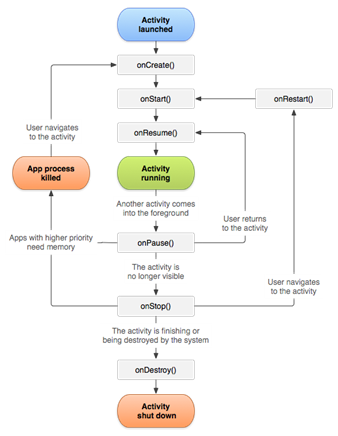
\includegraphics[scale=1]{Images/Figure-Example.png}
\caption{Acticity lifecycle}
\label{fig:activity-lifecycle}
\end{figure}

\clearpage

\begin{table}[!t]
\caption{Αριθμητικά δεδομένα}
\centering
\tabcolsep=0.5cm
\begin{adjustbox}{width=0.5 \textwidth}
    \begin{tabular}{|c|c|c|c|}
        \hline
        A/A & Τάση & Ρεύμα & Ισχύς \\ \hline
        1   & 33   & 45    & 333   \\ \hline
        2   & 45   & 54    & 565   \\ \hline
    \end{tabular}
\end{adjustbox}
\label{table:arithmetic-data}
\end{table}

Παραπάνω γίνεται αναφορά στον Πίνακας \ref{table:arithmetic-data}, όπου … .

\subsection{Μαθηματικές σχέσεις}
\label{subsection:rcpm2}
Οι μαθηματικές σχέσεις πρέπει να γράφονται με τη χρήση κατάλληλου λογισμικού και να αριθμούνται. Τα σύμβολα των μαθηματικών σχέσεων ορίζονται πάντοτε στη θέση που εισάγονται για πρώτη φορά. Η αρίθμηση των σχέσεων γίνεται μέσα σε παρενθέσεις, στο δεξί άκρο της σελίδας, ως εξής: Το πρώτο πεδίο αφορά τον αύξοντα αριθμό του κεφαλαίου όπου γράφεται η σχέση και το δεύτερο πεδίο τον αύξοντα αριθμό της σχέσης στο συγκεκριμένο κεφάλαιο. Ως παράδειγμα, η δεύτερη σχέση του πέμπτου κεφαλαίου φέρει την αρίθμηση (5.2), όπως παρακάτω που αναφέρεται στη σχέση (\ref{equation-1}):

\[F(x) = \int^a_b \frac{1}{3}x^3 \tag{3.1} \label{equation-1}\]

Η μαθηματική σχέση στοιχίζεται στο μέσο της σελίδας.

\subsection{Βιβλιογραφικές αναφορές} \label{subsection:rcpm-smote}
Οι βιβλιογραφικές αναφορές καταγράφονται με τη σειρά που παρατίθενται στο κείμενο, εντός αγκύλης [1], [2], [3] κλπ.

Για να προστεθεί στην βιβλιογραφία ένα βιβλίο, άρθρο, κ.τ.λ. πρέπει να εισαχθεί σε ένα αρχείο .bib σε μορφή BibTeX. Οι αναφορές στην βιβλιογραφία γίνονται μέσω τις εντολής \textbackslash cite, π.χ.: \cite{einstein}, \cite{sensory-receptors}, \cite{knuthwebsite}, \cite{knuth-fa}. Εφόσον η βιβλιογραφία χρησιμοποιεί την δομή της IEEE (\textbackslash bibliographystyle\{ieeetr\}), κάθε καταχώρηση θα εμφανιστεί με την σειρά στην οποία αναφέρθηκε στο κείμενο.

Κάθε βιβλιογραφική αναφορά στο κείμενο της εργασίας γίνεται με τον αριθμό της εντός αγκύλης, π.χ. \textbf{Ο πρώτος προσωπικός ηλεκτρονικός υπολογιστής της ΙΒΜ ήταν εμπορικά διαθέσιμος το 1981 \cite{sensory-receptors}}. Για την αναφορά περισσότερων από μιας πηγής, αναγράφονται όλες μαζί εντός αγκύλης, χωρισμένες μεταξύ τους με κόμμα π.χ. \textbf{\cite{latexcompanion, ctan},} εκτός αν είναι πολλές μαζί συνεχόμενες οπότε γράφονται στη μορφή [πρώτη – τελευταία], π.χ. \textbf{\cite{ctan, dirac, knuth-acp}}.


\subsection{Επίλογος} \label{chapter-3-conclusion}
Ο επίλογος ανακεφαλαιώνει τα κύρια σημεία του κάθε κεφαλαίου.

\clearpage

\section{Συμπεράσματα ή/και προτάσεις βελτίωσης} \label{chapter-4}

Σε αυτήν την ενότητα αναλύονται τα συμπεράσματα της διπλωματικής εργασίας και παρουσιάζονται προτάσεις βελτίωσης της.


\clearpage
\pagestyle{plain}
\nocite{*}
\bibliographystyle{ieeetr}

\renewcommand{\refname}{ΒΙΒΛΙΟΓΡΑΦΙΑ}
\addcontentsline{toc}{section}{ΒΙΒΛΙΟΓΡΑΦΙΑ}
\bibliography{bibliography}
\clearpage

\appendix
\titleformat{\section}
% Αλλαγή δομής των τίτλων των sections για τα παραρτήματα.
{\normalfont\large\bfseries}{ΠΑΡΑΡΤΗΜΑ Α:}{1em}{}

\section{ΤΙΤΛΟΣ ΠΑΡΑΡΤΗΜΑΤΟΣ}
Τα παραρτήματα μπορούν να είναι περισσότερα από ένα. Αριθμούνται με γράμματα του Ελληνικού αλφάβητου (Α, Β, Γ, …).

Στα παραρτήματα παρουσιάζονται πληροφορίες που δεν είναι κρίσιμες για την εργασία, αλλά σημαντικές για την απόδειξη συμπερασμάτων που αναπτύχθηκαν στην εργασία. Περιέχουν κώδικα λογισμικού, ερωτηματολόγια και απαντήσεις σε ερωτηματολόγια, κτλ.

\end{document}